\documentclass[11pt,a4paper]{article}
\usepackage[margin=2.0cm]{geometry}
\usepackage{amsmath,amssymb,booktabs,array,graphicx,tikz,float,hyperref}
\usetikzlibrary{arrows.meta,positioning,calc}
\hypersetup{colorlinks=true,linkcolor=blue!45!black,citecolor=blue!45!black,urlcolor=blue!45!black}
\def\UrlBreaks{\do\/\do-\do\_\do\.\do\?\do\=\do\&}
\setlength{\parskip}{0.28em}
\setlength{\parindent}{2em}
\graphicspath{{figures/}}

\definecolor{ink}{HTML}{203247}
\definecolor{muted}{HTML}{64778A}
\definecolor{teal}{HTML}{247A78}
\definecolor{orange}{HTML}{C56D54}
\definecolor{bluegray}{HTML}{5575A5}
\definecolor{pale}{HTML}{F4F7FA}
\definecolor{violet}{HTML}{7357A6}
\tikzset{
  flowpanel/.style={draw=ink!20,fill=white,rounded corners=2.2mm,line width=.65pt},
  paneltitle/.style={font=\sffamily\bfseries\small,text=ink},
  panelsub/.style={font=\sffamily\scriptsize,text=muted},
  flowarrow/.style={-{Stealth[length=2mm]},draw=ink!70,line width=1pt},
  graphedge/.style={draw=bluegray!60,line width=.75pt},
  focusedge/.style={draw=violet,line width=2.2pt},
  graphnode/.style={circle,draw=white,line width=.8pt,minimum size=5.6mm,inner sep=0pt,fill=bluegray},
  anomaly/.style={graphnode,fill=orange},
  gcnnode/.style={circle,draw=teal!70,fill=white,line width=1pt,minimum size=5.4mm,inner sep=0pt},
  explainernode/.style={circle,draw=violet!70,fill=white,line width=1pt,minimum size=5.2mm,inner sep=0pt}
}

\title{From Detection Performance to Explanation Fidelity: An Exploratory Evaluation on the GADBench Reddit Graph}
\author{}
\date{}

\begin{document}
\maketitle

\begin{abstract}
Graph neural networks (GNNs) use node attributes and neighborhood structure for anomaly detection. However, predictive performance does not establish explanation fidelity or causal validity. We used the SciencePrism controlled experiment runner to compare a two-layer graph convolutional network (GCN) with feature-only logistic regression on the GADBench Reddit graph. We also conducted an edge-mask deletion pilot on a fixed, small sample. Across three official splits of the same graph, mean AUPRC was $0.0620\pm0.0064$ for the GCN and $0.0605\pm0.0047$ for logistic regression. Mean AUROC was $0.6695\pm0.0197$ and $0.6594\pm0.0087$, respectively. These differences are descriptive because the splits share one graph. In the explanation pilot, 9 of 12 stratified test nodes from split 0 yielded explanations. The median difference in predicted-class logit drop between mask-ranked edges and 20 equal-size random deletions was $0.0025$. The mean was $0.4585$, driven largely by values near $1.377$ for three nodes labeled as normal, indicating substantial instance-level heterogeneity and precluding a general claim of explanation reliability. We distinguish detection labels, model-prediction perturbations, and explanation ground truth, and discuss limits arising from a single graph, transductive evaluation, a small explanation sample, and deletion-induced distribution shift.
\end{abstract}

\noindent\textbf{Keywords:} graph anomaly detection; graph neural networks; local explanations; fidelity; GADBench; GNNExplainer

\section{Introduction}
Node anomaly detection is complicated by severe class imbalance, interactions between node attributes and graph topology, and data-specific definitions of anomalous behavior. Graph neural networks combine node features with neighborhood information through message passing. Yet more complex GNNs do not necessarily outperform simpler neighborhood-aggregation or feature-based baselines in supervised graph anomaly detection. GADBench systematically compared 29 models across ten real-world graph datasets and found that simple tree ensembles remained competitive on several tasks\cite{tang2023gadbench}. GNN performance should therefore be established empirically rather than assumed.

Model explanations raise a question distinct from detection performance. GNNExplainer formulates the explanation of an individual prediction as an optimization problem over compact subgraphs and salient features\cite{ying2019gnnexplainer}. Highly weighted edges remain model-internal importance signals. A large prediction change after deleting them indicates sensitivity of the current output, but does not establish a causal anomaly mechanism. Studies of graph-explanation evaluation likewise show that conclusions depend on metric definitions, explanation targets, and perturbation distributions\cite{agarwal2022probing,zheng2024robust}.

Using the project-level SciencePrism controlled runner, we conducted a bounded exploratory evaluation on GADBench Reddit. We asked two questions:
\begin{enumerate}
  \item How do a two-layer GCN and feature-only logistic regression compare in AUPRC and AUROC under the same official splits?
  \item For a fixed sample of test nodes, how does deleting the top-$k$ mask-ranked edges change the predicted-class logit relative to deleting the same number of random edges?
\end{enumerate}
This study proposes neither a new detector nor a new explainer, and its single-graph results are not generalized to attributed graphs broadly. Dataset labels provide node-level ground truth for detection only; no edge-level explanation ground truth was available.

\section{Related Work}
\subsection{Graph Anomaly Detection}
Graph convolutional networks (GCNs) combine node attributes and local structure through layer-wise propagation over a normalized adjacency matrix\cite{kipf2017gcn}. GADBench benchmarks supervised graph anomaly detection across multiple models and real-world datasets\cite{tang2023gadbench}. We use its Reddit data and official train, validation, and test masks, with feature-only logistic regression as a narrow baseline. This comparison does not cover the full set of GADBench competitors and cannot reproduce the benchmark paper's model rankings.

\subsection{Local GNN Explanations and Fidelity}
GNNExplainer learns edge and feature masks to provide compact explanations for individual GNN predictions\cite{ying2019gnnexplainer}. Subsequent work emphasizes the need to specify the explanation target, evaluation protocol, and controls. Deletion-based fidelity metrics can also be affected by distribution shift in the perturbed graph\cite{agarwal2022probing,zheng2024robust}. Our local edge-mask pilot is inspired by GNNExplainer, but is neither a reproduction of the original method nor its official implementation. Random deletions serve only as a control for effects on the current prediction; they do not provide external labels for explanation correctness.

\section{Methods}
\subsection{Data and Splits}
We used the DGL Reddit graph file from the official GADBench repository\cite{gadbenchrepo}. The archived data contain 10,984 nodes, 64-dimensional node features, 366 anomaly labels, and 168,016 raw directed edge records. Graph semantics and label definitions follow the data source. The experiment script verifies the SHA-256 hash of the uncompressed source file on loading: \texttt{\scriptsize 575caca4\allowbreak 2abdb659\allowbreak cda70017\allowbreak 4854f7c1\allowbreak 542d0cb7\allowbreak f79f6766\allowbreak 12d4a838\allowbreak 5142a0fa}. The compressed input passed to the runner has a separate SHA-256 hash: \texttt{\scriptsize ce1ad69e\allowbreak a915d085\allowbreak 7495b7cc\allowbreak 75dc8853\allowbreak 5ac014b3\allowbreak 198f8213\allowbreak c7c35b09\allowbreak 347190d6}. These hashes refer to different file layers and should not be interchanged.

We trained and evaluated models separately under the three official train, validation, and test masks. Each mask-specific run used training labels for fitting, validation labels for early stopping or baseline selection, and test labels only for final AUPRC and AUROC calculation. We refer to these runs as split-level trials 0–2; random seeds 17–19 were assigned in order. Because all masks apply to the same graph, they are neither independent datasets nor evidence of cross-graph generalization. Feature transformations were fitted on training nodes only. The GCN used the full graph for transductive message passing, so test-node features and topology were visible during training, but test labels were not used for optimization.

\subsection{Detection Models}
The GCN had two layers and a hidden width of 32:
\begin{equation}
  H=\operatorname{ReLU}(\hat A X W_0),\qquad Z=\hat A H W_1,
\end{equation}
The adjacency matrix was symmetrized, binarized, and augmented with self-loops before symmetric degree normalization. We trained the model with class-weighted cross-entropy and Adam (learning rate, $0.01$; weight decay, $5\times10^{-4}$). Training stopped after at most 60 epochs, with early stopping after ten consecutive epochs without improved validation AUPRC. The three split-level trials used seeds 17, 18, and 19, respectively.

As a comparator, the baseline was logistic regression using node features only. The scaler was fitted on training nodes, and class-balanced weights were used during fitting. We selected $C\in\{0.1,1,10\}$ by validation AUPRC. Both models used the same masks, and test data did not inform model selection. We report AUPRC as the primary ranking metric for this imbalanced task and also report AUROC. Summary values are arithmetic means across the three split-level trials; $\pm$ denotes the sample standard deviation across masks. Because the trials share one graph and number only three, we performed no significance tests or independent-sample inference.

\subsection{Local Edge Masks and Deletion Controls}
The explanation pilot was restricted to split-level trial 0. Using a fixed random seed, we selected up to six anomalous and six normal test nodes, for a maximum of 12 candidates. For each node, we constructed a two-hop local subgraph and optimized a trainable mask shared across undirected edge pairs for 35 steps. The mask objective preserved the original predicted-class output while applying sparsity and entropy regularization. Candidate explanation edges were restricted to local edges incident to the target node's one-hop neighborhood. This implementation is an edge-mask variant inspired by GNNExplainer; it does not include the original method's full feature-mask objective or its official implementation.

We selected $k=\min(10,\max(1,\operatorname{round}(0.1m)))$ edges by mask logit, where $m$ is the number of candidate edges. For each node, we deleted the top-$k$ mask-ranked edges and 20 sets of the same number of randomly selected edges. Both deletion conditions retained the original graph's degree-normalization coefficients. We recorded the drop in the target model's logit for its \emph{predicted class}. We defined
\begin{equation}
  \Delta_i = d_i^{\mathrm{mask}} - \frac{1}{20}\sum_{j=1}^{20}d_{ij}^{\mathrm{random}}.
\end{equation}
Positive values indicate a larger predicted-class logit drop after deleting mask-ranked edges than after equal-size random deletion. $\Delta_i$ measures perturbation sensitivity for the current model and node; it is not explanation accuracy against ground truth. We skipped nodes when their two-hop subgraphs exceeded 3,000 nodes, the candidate-edge limit was exceeded, or too few candidate edges were available.

\begin{figure}[t]
\centering
\resizebox{\textwidth}{!}{%
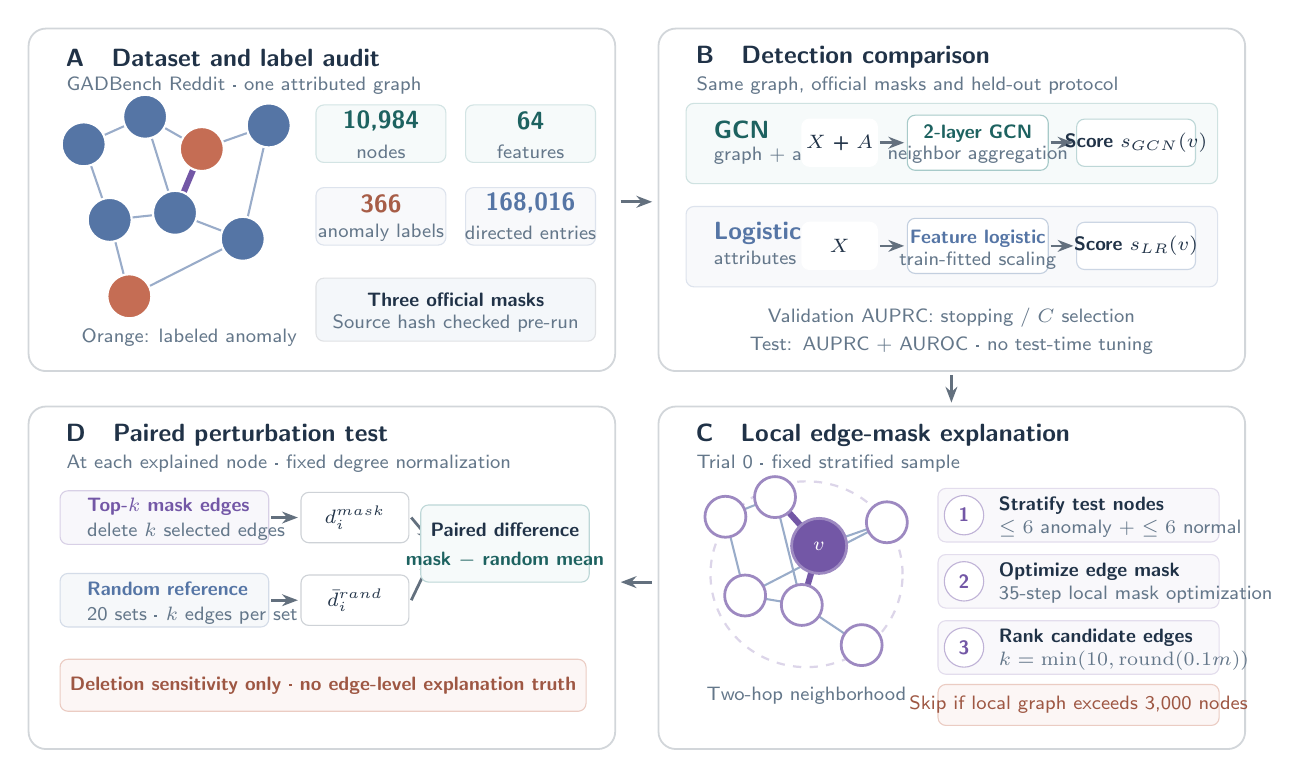
\begin{tikzpicture}[x=1cm,y=1cm,font=\sffamily]
  % A readable 2x2 sequence: audit -> compare -> explain -> perturb.
  \draw[flowpanel] (0,4.8) rectangle (7.45,9.15);
  \draw[flowpanel] (8,4.8) rectangle (15.45,9.15);
  \draw[flowpanel] (8,0) rectangle (15.45,4.35);
  \draw[flowpanel] (0,0) rectangle (7.45,4.35);
  \draw[flowarrow] (7.52,6.95)--(7.92,6.95);
  \draw[flowarrow] (11.72,4.75)--(11.72,4.40);
  \draw[flowarrow] (7.92,2.12)--(7.52,2.12);

  % A: audited graph and source facts.
  \node[paneltitle,anchor=west] at (.35,8.78) {A\quad Dataset and label audit};
  \node[panelsub,anchor=west] at (.36,8.43) {GADBench Reddit · one attributed graph};
  \draw[graphedge] (.70,7.68)--(1.48,8.03)--(2.20,7.62)--(3.05,7.92);
  \draw[graphedge] (.70,7.68)--(1.03,6.72)--(1.86,6.81)--(2.20,7.62);
  \draw[graphedge] (1.48,8.03)--(1.86,6.81)--(2.72,6.48)--(3.05,7.92);
  \draw[graphedge] (1.03,6.72)--(1.28,5.75)--(2.72,6.48);
  \draw[focusedge] (1.86,6.81)--(2.20,7.62);
  \node[graphnode] at (.70,7.68) {};
  \node[graphnode] at (1.48,8.03) {};
  \node[anomaly] at (2.20,7.62) {};
  \node[graphnode] at (3.05,7.92) {};
  \node[graphnode] at (1.03,6.72) {};
  \node[graphnode] at (1.86,6.81) {};
  \node[graphnode] at (2.72,6.48) {};
  \node[anomaly] at (1.28,5.75) {};
  \node[panelsub,anchor=west] at (.55,5.22) {Orange: labeled anomaly};

  \draw[draw=teal!20,fill=teal!4,rounded corners=1mm] (3.65,7.45) rectangle (5.30,8.18);
  \draw[draw=teal!20,fill=teal!4,rounded corners=1mm] (5.55,7.45) rectangle (7.20,8.18);
  \draw[draw=bluegray!20,fill=bluegray!4,rounded corners=1mm] (3.65,6.40) rectangle (5.30,7.13);
  \draw[draw=bluegray!20,fill=bluegray!4,rounded corners=1mm] (5.55,6.40) rectangle (7.20,7.13);
  \node[font=\sffamily\bfseries\small,text=teal!80!black] at (4.475,7.98) {10,984};
  \node[panelsub] at (4.475,7.59) {nodes};
  \node[font=\sffamily\bfseries\small,text=teal!80!black] at (6.375,7.98) {64};
  \node[panelsub] at (6.375,7.59) {features};
  \node[font=\sffamily\bfseries\small,text=orange!85!black] at (4.475,6.93) {366};
  \node[panelsub] at (4.475,6.56) {anomaly labels};
  \node[font=\sffamily\bfseries\small,text=bluegray] at (6.375,6.93) {168,016};
  \node[panelsub] at (6.375,6.56) {directed entries};
  \draw[draw=ink!14,fill=pale,rounded corners=1mm] (3.65,5.18) rectangle (7.20,5.98);
  \node[font=\sffamily\bfseries\scriptsize,text=ink,align=center] at (5.425,5.70) {Three official masks};
  \node[panelsub,align=center] at (5.425,5.40) {Source hash checked pre-run};

  % B: matched detector comparison.
  \node[paneltitle,anchor=west] at (8.35,8.78) {B\quad Detection comparison};
  \node[panelsub,anchor=west] at (8.36,8.43) {Same graph, official masks and held-out protocol};
  \draw[draw=teal!22,fill=teal!4,rounded corners=1mm] (8.35,7.18) rectangle (15.10,8.20);
  \draw[draw=bluegray!20,fill=bluegray!4,rounded corners=1mm] (8.35,5.87) rectangle (15.10,6.89);
  \node[font=\sffamily\bfseries\small,text=teal!80!black,anchor=west] at (8.58,7.86) {GCN};
  \node[panelsub,anchor=west] at (8.58,7.53) {graph + attributes};
  \draw[draw=white,fill=white,rounded corners=1mm] (9.82,7.40) rectangle (10.78,8.00);
  \node[font=\sffamily\bfseries\scriptsize,text=ink,align=center] at (10.30,7.70) {$X$ + $A$};
  \draw[flowarrow] (10.81,7.70)--(11.12,7.70);
  \draw[draw=teal!40,fill=white,rounded corners=1mm] (11.16,7.35) rectangle (12.95,8.05);
  \node[font=\sffamily\bfseries\scriptsize,text=teal!80!black] at (12.055,7.82) {2-layer GCN};
  \node[panelsub,align=center] at (12.055,7.55) {neighbor aggregation};
  \draw[flowarrow] (12.98,7.70)--(13.27,7.70);
  \draw[draw=teal!30,fill=white,rounded corners=1mm] (13.31,7.40) rectangle (14.82,8.00);
  \node[font=\sffamily\bfseries\scriptsize,text=ink,align=center] at (14.065,7.70) {Score $s_{GCN}(v)$};

  \node[font=\sffamily\bfseries\small,text=bluegray,anchor=west] at (8.58,6.55) {Logistic};
  \node[panelsub,anchor=west] at (8.58,6.22) {attributes only};
  \draw[draw=white,fill=white,rounded corners=1mm] (9.82,6.09) rectangle (10.78,6.69);
  \node[font=\sffamily\bfseries\scriptsize,text=ink,align=center] at (10.30,6.39) {$X$};
  \draw[flowarrow] (10.81,6.39)--(11.12,6.39);
  \draw[draw=bluegray!35,fill=white,rounded corners=1mm] (11.16,6.04) rectangle (12.95,6.74);
  \node[font=\sffamily\bfseries\scriptsize,text=bluegray,align=center] at (12.055,6.48) {Feature logistic};
  \node[panelsub,align=center] at (12.055,6.20) {train-fitted scaling};
  \draw[flowarrow] (12.98,6.39)--(13.27,6.39);
  \draw[draw=bluegray!30,fill=white,rounded corners=1mm] (13.31,6.09) rectangle (14.82,6.69);
  \node[font=\sffamily\bfseries\scriptsize,text=ink,align=center] at (14.065,6.39) {Score $s_{LR}(v)$};
  \node[panelsub,align=center,text width=6.3cm] at (11.72,5.48) {Validation AUPRC: stopping / $C$ selection};
  \node[panelsub,align=center,text width=6.3cm] at (11.72,5.12) {Test: AUPRC + AUROC · no test-time tuning};

  % C: local explainer applied to a fixed, stratified test sample.
  \node[paneltitle,anchor=west] at (8.35,3.98) {C\quad Local edge-mask explanation};
  \node[panelsub,anchor=west] at (8.36,3.63) {Trial 0 · fixed stratified sample};
  \draw[draw=violet!25,dashed,line width=.8pt] (9.88,2.22) ellipse (1.22 and 1.18);
  \draw[graphedge] (8.85,2.95)--(9.48,3.20)--(10.04,2.58)--(10.90,2.88);
  \draw[graphedge] (8.85,2.95)--(9.10,1.95)--(9.82,1.83)--(10.58,1.32);
  \draw[graphedge] (9.48,3.20)--(9.82,1.83)--(10.04,2.58);
  \draw[graphedge] (9.10,1.95)--(10.90,2.88);
  \draw[focusedge] (9.48,3.20)--(10.04,2.58);
  \draw[focusedge] (10.04,2.58)--(9.82,1.83);
  \node[explainernode] at (8.85,2.95) {};
  \node[explainernode] at (9.48,3.20) {};
  \node[explainernode,minimum size=7mm,fill=violet,text=white,font=\bfseries\scriptsize] at (10.04,2.58) {$v$};
  \node[explainernode] at (10.90,2.88) {};
  \node[explainernode] at (9.10,1.95) {};
  \node[explainernode] at (9.82,1.83) {};
  \node[explainernode] at (10.58,1.32) {};
  \node[panelsub,align=center] at (9.88,.68) {Two-hop neighborhood};

  \draw[draw=violet!20,fill=violet!4,rounded corners=1mm] (11.55,2.63) rectangle (15.12,3.31);
  \node[circle,draw=violet!45,fill=white,minimum size=5mm,inner sep=0pt,text=violet,font=\sffamily\bfseries\scriptsize] at (11.88,2.97) {1};
  \node[font=\sffamily\bfseries\scriptsize,text=ink,anchor=west] at (12.20,3.09) {Stratify test nodes};
  \node[panelsub,anchor=west] at (12.20,2.80) {$\leq 6$ anomaly + $\leq 6$ normal};
  \draw[draw=violet!20,fill=violet!4,rounded corners=1mm] (11.55,1.79) rectangle (15.12,2.47);
  \node[circle,draw=violet!45,fill=white,minimum size=5mm,inner sep=0pt,text=violet,font=\sffamily\bfseries\scriptsize] at (11.88,2.13) {2};
  \node[font=\sffamily\bfseries\scriptsize,text=ink,anchor=west] at (12.20,2.25) {Optimize edge mask};
  \node[panelsub,anchor=west] at (12.20,1.96) {35-step local mask optimization};
  \draw[draw=violet!20,fill=violet!4,rounded corners=1mm] (11.55,.95) rectangle (15.12,1.63);
  \node[circle,draw=violet!45,fill=white,minimum size=5mm,inner sep=0pt,text=violet,font=\sffamily\bfseries\scriptsize] at (11.88,1.29) {3};
  \node[font=\sffamily\bfseries\scriptsize,text=ink,anchor=west] at (12.20,1.41) {Rank candidate edges};
  \node[panelsub,anchor=west] at (12.20,1.12) {$k=\min(10,\operatorname{round}(0.1m))$};
  \draw[draw=orange!35,fill=orange!6,rounded corners=1mm] (11.55,.30) rectangle (15.12,.82);
  \node[panelsub,align=center,text=orange!80!black] at (13.335,.56) {Skip if local graph exceeds 3,000 nodes};

  % D: paired perturbation against equal-budget random deletion.
  \node[paneltitle,anchor=west] at (.35,3.98) {D\quad Paired perturbation test};
  \node[panelsub,anchor=west] at (.36,3.63) {At each explained node · fixed degree normalization};
  \draw[draw=violet!28,fill=violet!5,rounded corners=1mm] (.40,2.60) rectangle (3.05,3.28);
  \node[font=\sffamily\bfseries\scriptsize,text=violet,anchor=west] at (.62,3.08) {Top-$k$ mask edges};
  \node[panelsub,anchor=west] at (.62,2.76) {delete $k$ selected edges};
  \draw[draw=bluegray!25,fill=bluegray!5,rounded corners=1mm] (.40,1.55) rectangle (3.05,2.23);
  \node[font=\sffamily\bfseries\scriptsize,text=bluegray,anchor=west] at (.62,2.03) {Random reference};
  \node[panelsub,anchor=west] at (.62,1.69) {20 sets · $k$ edges per set};
  \draw[flowarrow] (3.08,2.94)--(3.42,2.94);
  \draw[flowarrow] (3.08,1.89)--(3.42,1.89);
  \draw[draw=ink!22,fill=white,rounded corners=1mm] (3.46,2.62) rectangle (4.83,3.26);
  \node[font=\sffamily\bfseries\scriptsize,text=ink,align=center] at (4.145,2.94) {$d_i^{mask}$};
  \draw[draw=ink!22,fill=white,rounded corners=1mm] (3.46,1.57) rectangle (4.83,2.21);
  \node[font=\sffamily\bfseries\scriptsize,text=ink,align=center] at (4.145,1.89) {$\bar d_i^{rand}$};
  \draw[flowarrow] (4.86,2.94)--(5.12,2.63);
  \draw[flowarrow] (4.86,1.89)--(5.12,2.43);
  \draw[draw=teal!30,fill=teal!4,rounded corners=1mm] (4.98,2.12) rectangle (7.12,3.10);
  \node[font=\sffamily\bfseries\scriptsize,text=ink,align=center] at (6.05,2.78) {Paired difference};
  \node[font=\sffamily\bfseries\scriptsize,text=teal!80!black,align=center] at (6.05,2.40) {mask $-$ random mean};
  \draw[draw=orange!35,fill=orange!6,rounded corners=1mm] (.40,.48) rectangle (7.08,1.14);
  \node[font=\sffamily\bfseries\scriptsize,text=orange!80!black,align=center] at (3.74,.81) {Deletion sensitivity only · no edge-level explanation truth};
\end{tikzpicture}%
}
\caption{Study workflow and the scope of explanation evaluation. (A) Audited GADBench Reddit input. (B) Transductive GCN and feature-only logistic regression evaluated under the same official splits. (C) Local edge-mask optimization on a fixed, stratified sample from split-level trial 0. (D) Effects on the predicted-class logit after deleting the top-$k$ mask-ranked edges or the same number of random edges. Arrows indicate the analysis sequence. Perturbation effects are not explanation ground truth.}
\label{fig:framework}
\end{figure}

\section{Results}
\subsection{Detection Performance}
Table~\ref{tab:detection} summarizes test performance across the three official splits. The test set in split-level trial 0 contained 4,395 nodes, including 147 anomalies (3.34\%). GCN AUPRC was higher than logistic-regression AUPRC in trials 0 and 2, but lower in trial 1. AUROC showed the same direction of split-wise variation. The mean differences across trials were $0.0016$ in AUPRC and $0.0101$ in AUROC. Because the three splits share one underlying graph, these differences are descriptive and do not provide statistical evidence of GCN superiority.

\begin{table}[t]
\centering
\small
\caption{Detection metrics across the official splits. The summary row reports the mean and sample standard deviation across three split-level trials. LR denotes feature-only logistic regression.}
\label{tab:detection}
\begin{tabular}{c r r r r}
\toprule
Split-level trial & GCN AUPRC & LR AUPRC & GCN AUROC & LR AUROC\\
\midrule
Trial 0 & 0.0694 & 0.0610 & 0.6917 & 0.6669\\
Trial 1 & 0.0588 & 0.0649 & 0.6541 & 0.6615\\
Trial 2 & 0.0578 & 0.0555 & 0.6627 & 0.6499\\
\midrule
Mean $\pm$ SD & $0.0620\pm0.0064$ & $0.0605\pm0.0047$ & $0.6695\pm0.0197$ & $0.6594\pm0.0087$\\
\bottomrule
\end{tabular}
\end{table}

\subsection{Local Explanation Perturbations}
Explanation optimization succeeded for 9 of the 12 sampled nodes. Three nodes were skipped because their two-hop subgraphs exceeded 3,000 nodes. Four of the nine successfully explained nodes carried anomaly labels, and five carried normal labels. Across these nodes, the mean $\Delta_i$ was $0.4585$ (sample SD, $0.6891$), and the median was $0.0025$. Mean $\Delta_i$ was $-0.0015$ for anomaly-labeled nodes ($n=4$) and $0.8264$ for nodes labeled as normal ($n=5$). Three nodes labeled as normal contributed values near $1.377$; the other six successful cases were close to zero. The overall mean therefore does not represent a typical node effect and should not be interpreted as general explanation fidelity.

Figure~\ref{fig:results} shows split-wise detection metrics alongside node-wise perturbation differences. Panel C retains the full range across all successful cases. Panel D expands the scale for the six remaining near-zero cases so that three large values do not compress the other points. A positive difference indicates a larger predicted-class logit drop after deleting mask-ranked edges than after random deletion. It measures sensitivity of this model to the specified perturbation only.

\begin{figure}[t]
\centering
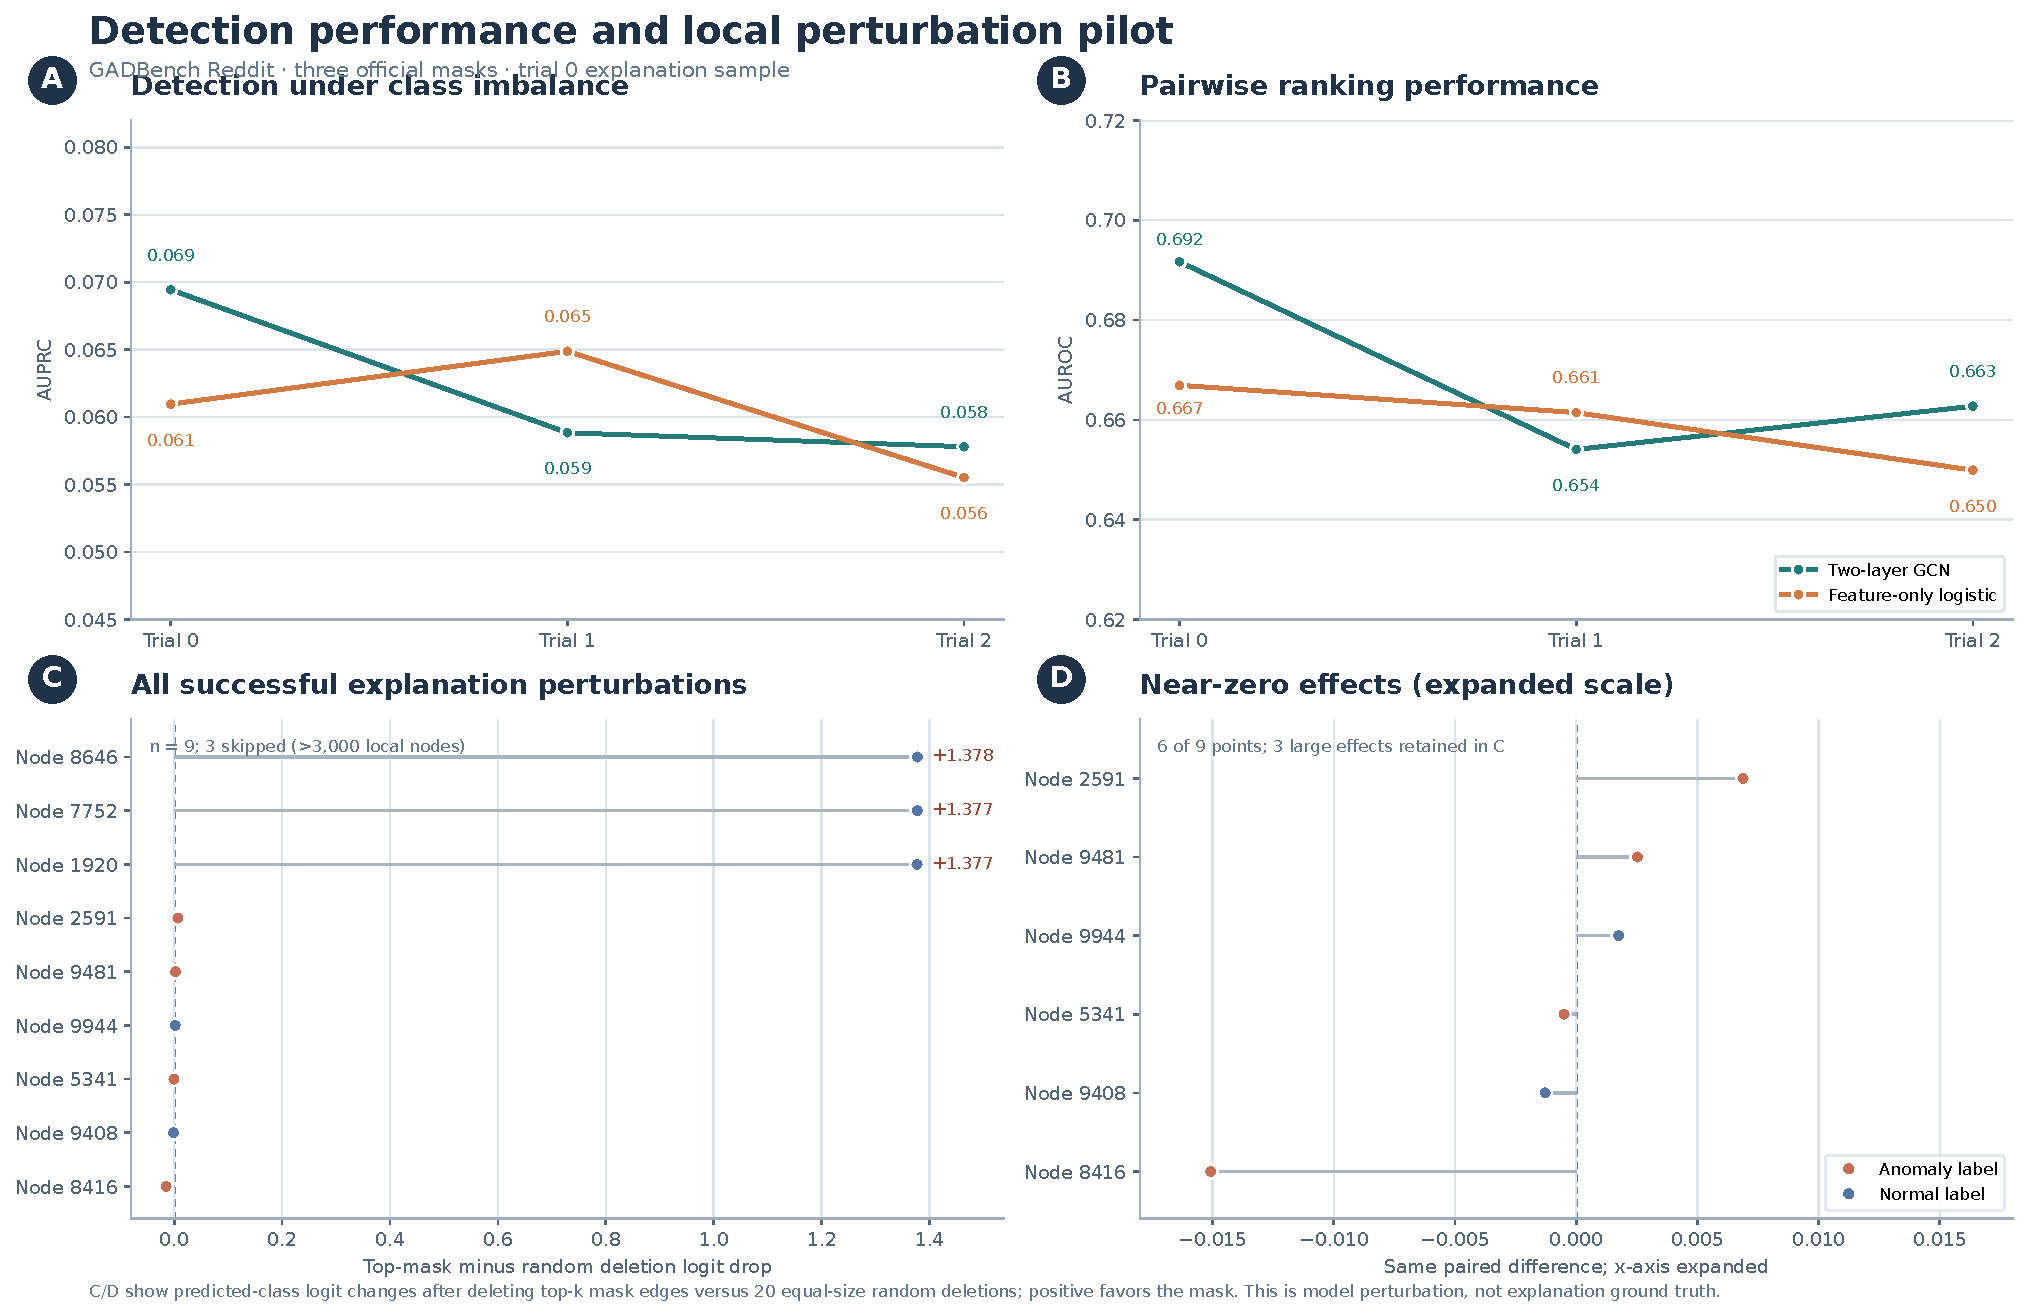
\includegraphics[width=\textwidth]{figure2-gadbench-results.pdf}
\caption{Detection and local perturbation results on GADBench Reddit. (A,B) AUPRC and AUROC under the three official masks. Lines connect split-wise results for the same model and do not represent a temporal trend or independent replication. (C) Full paired differences for nine successfully explained nodes. (D) Expanded view of the six nodes with absolute differences below 0.05; the three larger values remain visible in C. Colors distinguish anomaly and normal labels. Perturbation differences are not explanation ground truth.}
\label{fig:results}
\end{figure}

\section{Discussion}
The two-layer GCN and feature-only logistic regression had similar mean metrics, and the GCN did not lead on every split. This observation is consistent with GADBench's rationale for evaluating simple baselines broadly. However, a comparison on one dataset cannot support conclusions about model rankings across GADBench. Reddit has a low anomaly prevalence, making AUPRC sensitive to performance on the minority class. AUROC alone may also obscure precision constraints at low prevalence.

The explanation pilot showed a strongly skewed distribution of differences between mask-ranked and random deletions. The median was close to zero, whereas three large values from nodes labeled as normal raised the mean. Reporting only the aggregate mean would therefore obscure the small effects in most cases. A normal label does not imply a normal model prediction. Our perturbations targeted the model's current predicted-class logit, and node labels were not used to optimize edge masks. The observed differences establish neither an anomaly mechanism nor the semantic correctness of the masks.

The explanation benchmark is also limited by its implementation and perturbation protocol. Its objective is a simplified GNNExplainer-inspired variant, not a reproduction of the original method. The pilot included only 12 prespecified nodes, and three explanations could not be generated because of local-subgraph size limits. All deletions retained the original degree-normalization coefficients, so perturbed graphs differed from graphs that would be obtained by recomputing normalization. Deletion may also create structures outside the training distribution. Future studies could evaluate more independent graphs and explanation instances using robust perturbation protocols. They could also separate model fidelity from mechanistic correctness using data with trusted edge annotations or synthetic ground truth.

\section{Limitations}
Five limitations bound the conclusions. First, the experiment used one Reddit graph and one two-layer GCN, so it does not represent attributed graphs or graph anomaly-detection methods broadly. Second, the three official masks share the same nodes, features, and topology. Their across-split standard deviation is not cross-dataset uncertainty and should not be treated as a confidence interval from independent samples. Third, transductive message passing exposed the model to full-graph structure and test-node features during training. Test labels were withheld, but this setting differs from inductive prediction on new graphs. Fourth, local explanations covered a small, fixed sample from split-level trial 0, with size-related exclusions. Fifth, the dataset provides detection labels but no edge-level explanation ground truth. Perturbation therefore measures local model sensitivity only, and fixed degree normalization plus deletion-induced distribution shift may affect that measure. The findings should consequently be interpreted as exploratory.

\section{Conclusion}
Across the three official GADBench Reddit splits, the two-layer GCN and feature-only logistic regression achieved similar detection metrics with split-wise variation. The small mask-deletion pilot had a near-zero median difference and a few large positive outliers, illustrating why instance-level results are more informative than a single mean. The evidence neither establishes consistent GCN superiority under this setting nor shows that local explanations reveal real anomaly causes. Reliable conclusions about explainable graph anomaly detection require more independent graphs, broader instance-level evaluation, and trusted explanation ground truth.

\section*{Data and Code Availability}
The experiment was executed with the SciencePrism controlled runner. The run ID is \path{experiment-run-bca97a65-c447-4e18-87d0-e267623c78ec}.

The run manifest, environment record, standard output, standard error, \texttt{metrics.json}, and \texttt{results.json} are stored in the project archive at \path{.scienceprism/experiment-runs/}.

Byte-identical copies of the manifest, environment record, standard output, standard error, \texttt{metrics.json}, and \texttt{results.json} are included in the repository under \path{docs/research/run-artifacts/}. The results figure can be regenerated from \texttt{results/results.json} with \path{docs/research/plot-gadbench-results.py}. The model and data-preparation scripts are available at \path{experiments/reddit_gcn_explain.py} and \path{scripts/prepare-gadbench-reddit.py}, respectively. GADBench source code and data are available from the official repository\cite{gadbenchrepo}.

To avoid redistributing the raw dataset, the archive records hashes for the compressed project input and the original source file. This study did not independently conduct a legal review of the dataset license or all associated metadata.

\begin{thebibliography}{9}
\bibitem{tang2023gadbench}
Tang J, Hua F, Gao Z, Zhao P, Li J. GADBench: Revisiting and Benchmarking Supervised Graph Anomaly Detection. In: \emph{Advances in Neural Information Processing Systems}; 2023.\newline
\href{https://proceedings.neurips.cc/paper_files/paper/2023/hash/5eaafd67434a4cfb1cf829722c65f184-Abstract-Datasets_and_Benchmarks.html}{NeurIPS 2023 paper page}

\bibitem{ying2019gnnexplainer}
Ying Z, Bourgeois D, You J, Zitnik M, Leskovec J. GNNExplainer: Generating Explanations for Graph Neural Networks. In: \emph{Advances in Neural Information Processing Systems}; 2019.\newline
\href{https://proceedings.neurips.cc/paper/2019/hash/d80b7040b773199015de6d3b4293c8ff-Abstract.html}{NeurIPS 2019 paper page}

\bibitem{kipf2017gcn}
Kipf TN, Welling M. Semi-Supervised Classification with Graph Convolutional Networks. In: \emph{International Conference on Learning Representations}; 2017.\newline
\href{https://openreview.net/pdf?id=SJU4ayYgl}{ICLR 2017 paper PDF}

\bibitem{agarwal2022probing}
Agarwal C, Zitnik M, Lakkaraju H. Probing GNN Explainers: A Rigorous Theoretical and Empirical Analysis of GNN Explanation Methods. In: \emph{Proceedings of AISTATS}; 2022;151:8969--8996.\newline
\href{https://proceedings.mlr.press/v151/agarwal22b.html}{PMLR paper page}

\bibitem{zheng2024robust}
Zheng X, Shirani F, Wang T, Cheng W, Chen Z, Chen H, Wei H, Luo D. Towards Robust Fidelity for Evaluating Explainability of Graph Neural Networks. In: \emph{International Conference on Learning Representations}; 2024.\newline
\href{https://proceedings.iclr.cc/paper_files/paper/2024/hash/34293d684b1012ed45c3274b4a7edc00-Abstract-Conference.html}{ICLR 2024 paper page}

\bibitem{gadbenchrepo}
Tang J, et al. GADBench official code and dataset repository.\newline
\url{https://github.com/squareRoot3/GADBench}
\end{thebibliography}

\end{document}
